\documentclass{article}
% Chinese
% \documentclass[UTF8, nofonts, mathptmx, 12pt, onecolumn]{article}
% \usepackage{xeCJK}
% \setCJKmainfont{SimSun}
\usepackage{amsmath}
\usepackage{amsfonts}
\usepackage{amssymb}
\usepackage{wasysym}
% \usepackage{ctex}
\usepackage{graphicx}
\usepackage{float}
\usepackage{geometry}
\geometry{a4paper,scale=0.8}
\usepackage{caption}
\usepackage{subcaption}
% \newcommand{\oiint}{\mathop{{\int\!\!\!\!\!\int}\mkern-21mu \bigcirc} {}}
\newcommand*{\dif}{\mathop{}\!\mathrm{d}}
\newcommand*{\md}{\mathop{}\!\mathrm{d}}
\newcommand*{\me}{\mathrm{e}}

% \usepackage{parskip}
% \setlength{\parindent}{0cm}

\usepackage{bm}
\let\Oldmathbf\mathbf
\renewcommand{\mathbf}[1]{\boldsymbol{\Oldmathbf{#1}}}
\let\eqnarray\align

\author{Xiping Hu}
\usepackage{authblk}
\author{Xiping Hu}
\affil{https://hxp.plus/}
\title{Homework for Chapter 2}

\begin{document}
\maketitle

\begin{figure}[H]
  \centering
  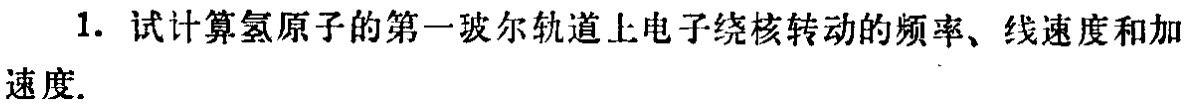
\includegraphics[width=\linewidth]{figures/Problem1}
  \label{fig:}
\end{figure}

\begin{equation*}
  \begin{aligned}
  \end{aligned}
\end{equation*}
\begin{equation*}
  \begin{aligned}
    r_0 &= \dfrac{4 \pi \varepsilon_0 \hbar^2}{m_e e^2} \\
    V_1 &= \alpha c = \dfrac{c}{137} = 2.19 \times 10^6 \  \mathrm{m/s} \\
    \nu &= \dfrac{2 \pi r_0}{V_1} = 6.58 \times 10^{15} \  \mathrm{Hz} \\
    a &= \dfrac{V_1^2}{r_0} = 9.046 \times 10^{22} \  \mathrm{m/s^2}
  \end{aligned}
\end{equation*}

\begin{figure}[H]
  \centering
  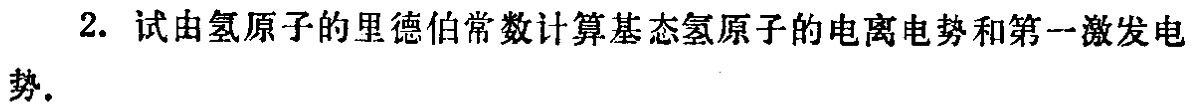
\includegraphics[width=\linewidth]{figures/Problem2}
  \label{fig:}
\end{figure}

The energy of atom at different state are

\begin{equation*}
  \begin{aligned}
    E_1 &= - hc R_H = -13.6 \  \mathrm{eV} \\
    E_2 &= - hc R_H \dfrac{1}{2^2} = -3.4 \  \mathrm{eV} \\
  \end{aligned}
\end{equation*}
\begin{equation*}
  \begin{aligned}
    E_2 - E_1 &= 10.2 \  \mathrm{eV}
  \end{aligned}
\end{equation*}



So that the Ionization potential is $13.6 \  \mathrm{eV}$, the First excitation potential is $10.2 \  \mathrm{eV}$

\begin{figure}[H]
  \centering
  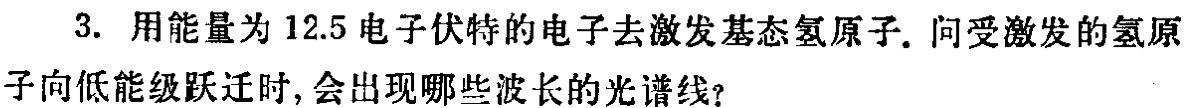
\includegraphics[width=\linewidth]{figures/Problem3}
  \label{fig:}
\end{figure}

\begin{equation*}
  \begin{aligned}
    E_2 &= hc R_H \left( 1 - \dfrac{1}{2^2} \right) = 10.2 \  \mathrm{eV} \\
    E_3 &= hc R_H \left( 1 - \dfrac{1}{3^2} \right) = 12.1 \  \mathrm{eV} \\
  \end{aligned}
\end{equation*}
\begin{equation*}
  \begin{aligned}
    E_4 &= hc R_H \left( 1 - \dfrac{1}{4^2} \right) = 12.8 \  \mathrm{eV}
  \end{aligned}
\end{equation*}

So that the maximum state the atom may reach is $3$, possible wavelength of emitted light during transition are:

\begin{equation*}
  \begin{aligned}
    \lambda_1 = \dfrac{1}{R_H \left( \dfrac{1}{1^2} - \dfrac{1}{3^2} \right)} = 1.025 \times 10^{-7} \  \mathrm{m} \\
    \lambda_2 = \dfrac{1}{R_H \left( \dfrac{1}{1^2} - \dfrac{1}{2^2} \right)} = 1.215 \times 10^{-7} \  \mathrm{m} \\
    \lambda_3 = \dfrac{1}{R_H \left( \dfrac{1}{2^2} - \dfrac{1}{3^2} \right)} = 6.565 \times 10^{-7} \  \mathrm{m} \\
  \end{aligned}
\end{equation*}

\begin{figure}[H]
  \centering
  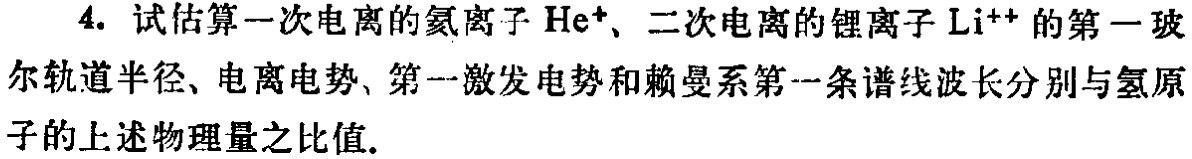
\includegraphics[width=\linewidth]{figures/Problem4}
  \label{fig:}
\end{figure}

\begin{equation*}
  \begin{aligned}
    r_n &= a_0 \cdot \dfrac{n^2}{Z} \\
    E_n &= - \dfrac{m_e e^4}{2 \left( 4 \pi \varepsilon_0 \hbar \right)^2} \cdot \dfrac{Z^2}{n^2}  \\
    \nu &= Z^2 R \left( \dfrac{1}{n_1} - \dfrac{1}{n_2}   \right)
  \end{aligned}
\end{equation*}

So that

\begin{equation*}
  \begin{aligned}
    \dfrac{r_{He}}{r_H} = \dfrac{1}{2} \\
    \dfrac{r_{Li}}{r_H} = \dfrac{1}{3}  
  \end{aligned}
\end{equation*}

\begin{equation*}
  \begin{aligned}
    \dfrac{E_{He}_1}{E_H_1} = \dfrac{4}{1} \\
    \dfrac{E_{Li}_1}{E_H_1} = \dfrac{9}{1}  
  \end{aligned}
\end{equation*}
\begin{equation*}
  \begin{aligned}
    \dfrac{E_{He}_2 - E_{He}_1}{E_H_2 - E_H_1} = 4 \\
    \dfrac{E_{Li}_2 - E_{Li}_1}{E_H_2 - E_H_1} = 9 
  \end{aligned}
\end{equation*}
\begin{equation*}
  \begin{aligned}
    \dfrac{\nu_{He}}{\nu_H} = 4 \\
    \dfrac{\nu_{Li}}{\nu_H} = 9 
  \end{aligned}
\end{equation*}

\begin{figure}[H]
  \centering
  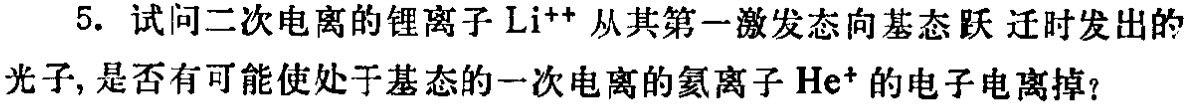
\includegraphics[width=\linewidth]{figures/Problem5}
  \label{fig:}
\end{figure}

\begin{equation*}
  \begin{aligned}
    E_{Li}_2 - E_{Li}_1 = \dfrac{9}{2} R
  \end{aligned}
\end{equation*}
\begin{equation*}
  \begin{aligned}
    E_{He}_1 = 4 R \leq \dfrac{9}{2} R 
  \end{aligned}
\end{equation*}

The photon emitted by $Li^{2+}$ can ionize $He^+$.

\begin{figure}[H]
  \centering
  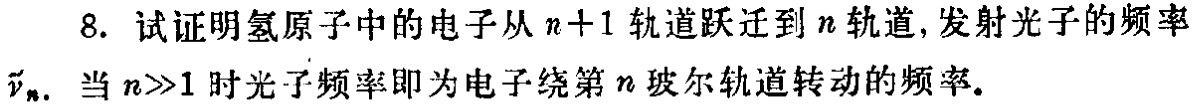
\includegraphics[width=\linewidth]{figures/Problem8}
  \label{fig:}
\end{figure}

\begin{equation*}
  \begin{aligned}
    \nu &= R_H \left[ \dfrac{1}{n} - \dfrac{1}{n + 1}  \right] \\
    &= \dfrac{2 \pi^2 e^4 m}{\left( 4 \pi \varepsilon_0 \right)^2 h^3 c} \left[ \dfrac{1}{n^2} - \dfrac{1}{\left( n + 1 \right)^2}  \right] \\
    &= \dfrac{2 \pi^2 e^4 m}{\left( 4 \pi \varepsilon_0 \right)^2 h^3 c} \cdot \left[\dfrac{\md}{\md n}\left( \dfrac{1}{n^2}  \right)  \right] \left[ n - \left( n + 1 \right) \right]\\
    &= \dfrac{4 \pi^2 e^4 m}{\left( 4 \pi \varepsilon_0 \right)^2 h^3 c} \cdot \dfrac{1}{n^3} 
  \end{aligned}
\end{equation*}
\begin{equation*}
  \begin{aligned}
    \dfrac{1}{T} =  \dfrac{V}{2 \pi r} = \dfrac{\alpha c}{2 \pi a_0} \cdot \dfrac{1}{n^3} = \dfrac{c}{2 \pi} \cdot \dfrac{m e^4}{4 \pi \varepsilon_0 \hbar c \cdot 4 \pi \varepsilon_0 \hbar^2} \cdot \dfrac{1}{n^3} = \nu
  \end{aligned}
\end{equation*}

\begin{figure}[H]
  \centering
  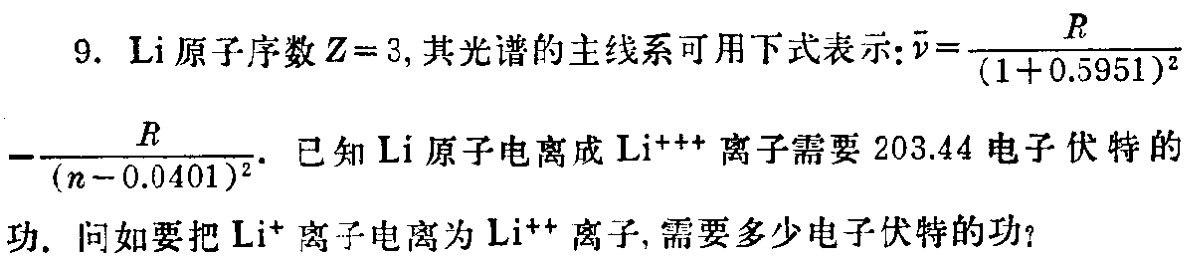
\includegraphics[width=\linewidth]{figures/Problem9}
  \label{fig:}
\end{figure}

Assume that the energy needed to transfer $Li$ to $Li^+$ is $E_1$, the energy to transfer $Li^+$ to $Li^{2+}$ is $E_2$, and the energy to transfer $Li^{2+}$ to $Li^{3+}$ is $E_3$.

\begin{equation*}
  \begin{aligned}
    E_1 + E_2 + E_3 = 203.44 \  \mathrm{eV}
  \end{aligned}
\end{equation*}
\begin{equation*}
  \begin{aligned}
    E_1 &= \lim_{n \rightarrow \infty} \left[ \dfrac{R}{\left( 1 + 0.5901 \right)^2} - \dfrac{R}{\left( 1 - 0.0401 \right)^2}   \right] \cdot h c = 5.35 \  \mathrm{eV}
  \end{aligned}
\end{equation*}
\begin{equation*}
  \begin{aligned}
    E_3 &= 9 R h c = 122.4 \  \mathrm{eV}
  \end{aligned}
\end{equation*}
\begin{equation*}
  \begin{aligned}
    E_2 = 203.44 - E_1 - E_2 = 75.7 \  \mathrm{eV}
  \end{aligned}
\end{equation*}

\begin{figure}[H]
  \centering
  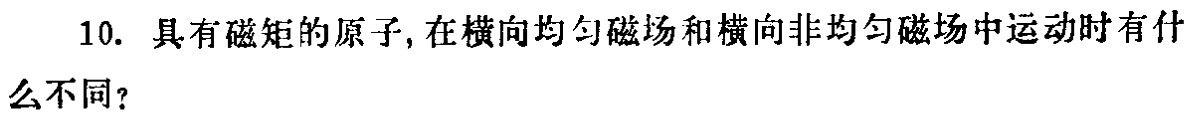
\includegraphics[width=\linewidth]{figures/Problem10}
  \label{fig:}
\end{figure}

In an uniformed magnet field, where $\dfrac{\md B}{\md z} = 0 $, no force will be applied on the atom. And the electron will move around the nucleus in an qumntumized, eclipse shaped orbit. Also, precession of the orbit will take place if relativity is concerned.

In a varied magnet field, where $\dfrac{\md B}{\md z} \neq 0 $, besides the motion described above, magnetic force will be applied to the atom.

\begin{figure}[H]
  \centering
  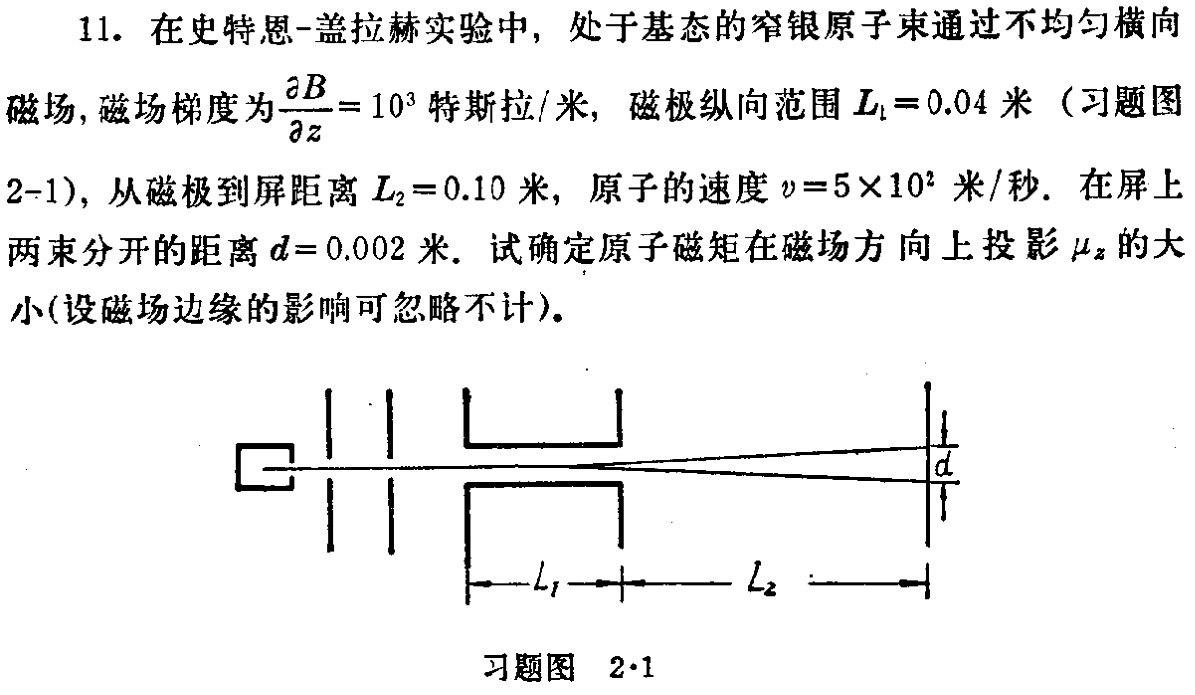
\includegraphics[width=\linewidth]{figures/Problem11}
  \label{fig:}
\end{figure}

\begin{equation*}
  \begin{aligned}
    f = \mu_z \dfrac{\md B}{\md z} 
  \end{aligned}
\end{equation*}
\begin{equation*}
  \begin{aligned}
    a = \dfrac{f}{m} = \dfrac{1}{m} \cdot \dfrac{\md B}{\md z} \cdot \mu_z
  \end{aligned}
\end{equation*}
\begin{equation*}
  \begin{aligned}
    t_1 = \dfrac{L_1}{v} \\
    t_2 = \dfrac{L_2}{v} 
  \end{aligned}
\end{equation*}

\begin{equation*}
  \begin{aligned}
    S_1 = \dfrac{1}{2} a t_1^2 = \dfrac{1}{2 m} \cdot \left( \dfrac{L_1}{v} \right) \cdot \dfrac{\md B}{\md z} \cdot \mu_z 
  \end{aligned}
\end{equation*}
\begin{equation*}
  \begin{aligned}
    S_2 = a t_1 t_2 = \dfrac{1}{m} \cdot \dfrac{\md B}{\md z} \cdot \dfrac{L_1 L_2}{v^2} \cdot \mu_z 
  \end{aligned}
\end{equation*}
\begin{equation*}
  \begin{aligned}
    S_1 + S_2 = \dfrac{d}{2}
  \end{aligned}
\end{equation*}
\begin{equation*}
  \begin{aligned}
    \dfrac{1}{2 m} \cdot \left( \dfrac{L_1}{v} \right) \cdot \dfrac{\md B}{\md z} \cdot \mu_z + \dfrac{1}{m} \cdot \dfrac{\md B}{\md z} \cdot \dfrac{L_1 L_2}{v^2} \cdot \mu_z = \dfrac{d}{2} 
  \end{aligned}
\end{equation*}
\begin{equation*}
  \begin{aligned}
    \dfrac{1}{2m} \cdot \dfrac{L_1 \left( L_1 + 2 L_2 \right)}{v^2} \cdot \dfrac{\md B}{\md z} \cdot \mu_z = \dfrac{d}{2}   
  \end{aligned}
\end{equation*}
\begin{equation*}
  \begin{aligned}
    \mu_z = 9.3 \times 10^{-24} \  \mathrm{J \cdot T^{-1}}
  \end{aligned}
\end{equation*}










\end{document}